\begin{frame}{Learning objectives}
\begin{itemize}
\item Model a binary outcome using logistic regression.
\item Translate between probabilities, odds and log-odds.
\item Interpret coefficients and odds ratios with their limitations.
\item Choose a decision threshold using validation data.
\item Evaluate discrimination, calibration and decision errors.
\end{itemize}
\end{frame}

\begin{frame}{A binary target}
\begin{itemize}
\item A delivery is on time ($Y=0$) or late ($Y=1$).
\item We want $p(\mathbf x)=P(Y=1\mid\mathbf X=\mathbf x)$.
\item Available predictors: distance and peak-time dispatch.
\item The outcome coding must be explicit: reversing 0 and 1 reverses the event being modelled.
\end{itemize}
\end{frame}

\begin{frame}{Why not use an unconstrained line?}
\begin{itemize}
\item A linear probability prediction can fall below 0 or above 1.
\item For Bernoulli outcomes, conditional variance is $p(1-p)$, not constant.
\item A constant change in probability across the whole predictor range may be implausible.
\item The logistic link constrains predictions to the probability scale.
\end{itemize}
\end{frame}

\begin{frame}{Probability, odds and log-odds}
\[\text{odds}=\frac{p}{1-p},\qquad\operatorname{logit}(p)=\log\frac{p}{1-p}.\]\begin{center}\begin{tabular}{rrr}\toprule
$p$ & Odds & Log-odds\\\midrule 0.20 & 0.25 & -1.386\\0.50 & 1.00 & 0.000\\0.80 & 4.00 & 1.386\\
\bottomrule\end{tabular}\end{center}Odds compare the probability of the event with the probability of its complement.
\end{frame}

\begin{frame}{The logistic regression model}
\[\log\frac{p(\mathbf x)}{1-p(\mathbf x)}=\eta=\beta_0+\sum_{j=1}^p\beta_jx_j.\]\[\boxed{p(\mathbf x)=\frac{e^\eta}{1+e^\eta}=\frac{1}{1+e^{-\eta}}}\]The model is linear in log-odds, while the probability response is nonlinear.
\end{frame}

\begin{frame}{A worked probability calculation}
Use the illustrative model\[\eta=-3+0.18\,\text{distance}+0.9\,\text{peak}.\]\begin{center}\begin{tabular}{lrr}\toprule
10 km delivery & Off peak & Peak\\\midrule $\eta$ & -1.2 & -0.3\\ $p=1/(1+e^{-\eta})$ & 0.2315 & 0.4256\\
\bottomrule\end{tabular}\end{center}These are specified teaching coefficients, not estimates from the sample.
\end{frame}

\begin{frame}{Probability curves}
\centering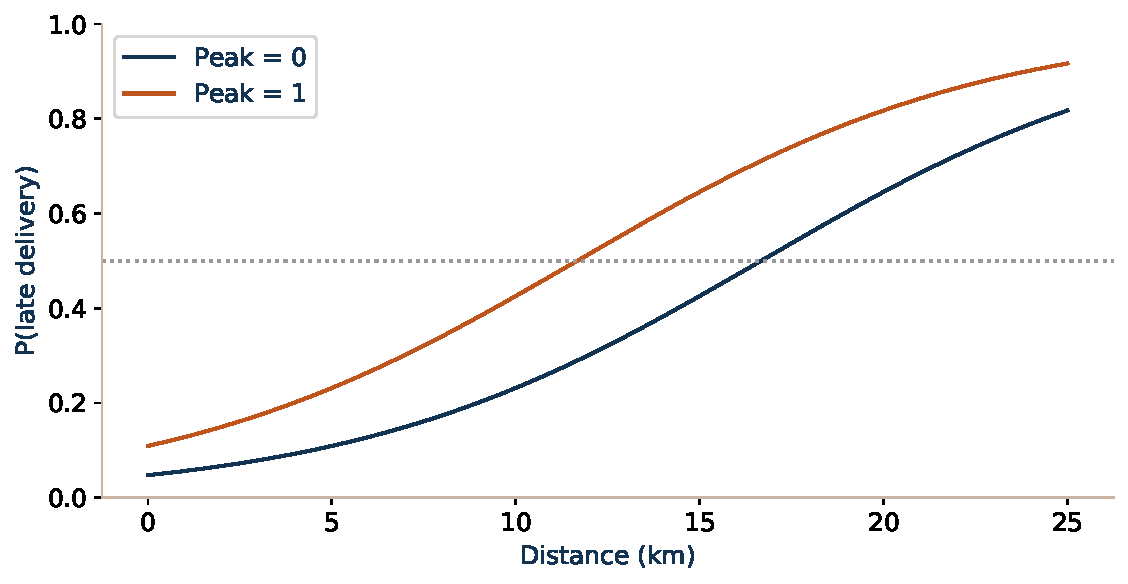
\includegraphics[width=.86\textwidth,height=.64\textheight,keepaspectratio]{figures/supervised/logistic_curves.pdf}
\end{frame}

\begin{frame}{Interpreting a coefficient}
\[\frac{\text{odds at }x_j+1}{\text{odds at }x_j}=e^{\beta_j}.\]\begin{itemize}
\item Hold all other included predictors fixed.
\item For distance, $e^{0.18}=1.197$: the odds are about 19.7\% higher per km.
\item For peak time, $e^{0.9}=2.460$: the odds are about 2.46 times as large.
\item This is not a constant increase in probability and is not automatically causal.
\end{itemize}
\end{frame}

\begin{frame}{Odds ratios are not risk ratios}
If $p_0=0.20$, then initial odds are $0.25$. An odds ratio of 2 gives\[\text{new odds}=0.50,\qquad p_1=\frac{0.50}{1+0.50}=0.3333.\]\begin{itemize}
\item Probability rises from 20\% to 33.3\%, not 40\%.
\item The probability ratio is $0.3333/0.20=1.667$, not 2.
\item The probability difference depends on the starting probability.
\end{itemize}
\end{frame}

\begin{frame}{Marginal probability effects}
With no interaction or transformation for $x_j$,\[\frac{\partial p}{\partial x_j}=\beta_jp(1-p).\]\begin{itemize}
\item The probability effect is largest in magnitude near $p=0.5$.
\item The same coefficient can imply small changes near 0 or 1.
\item For a binary predictor, compare predicted probabilities at 0 and 1 rather than taking a derivative.
\end{itemize}
\end{frame}

\begin{frame}{How coefficients are estimated}
For independent Bernoulli outcomes,\[L(\boldsymbol\beta)=\prod_i p_i^{y_i}(1-p_i)^{1-y_i}.\]\[\ell(\boldsymbol\beta)=\sum_i\{y_i\log p_i+(1-y_i)\log(1-p_i)\}.\]\begin{itemize}
\item Maximum likelihood selects coefficients that maximise this log-likelihood.
\item Equivalently, it minimises average log loss.
\item Unlike simple OLS, the solution is generally found iteratively.
\end{itemize}
\end{frame}

\begin{frame}{Assumptions and estimation problems}
\begin{itemize}
\item Specify the event and a plausible relationship linear in log-odds.
\item Account for dependence, clustering and sampling where relevant.
\item Avoid exact linear dependence among predictors.
\item Complete or quasi-complete separation can lead to infinite estimates.
\item Very rare events and small samples can make estimates and intervals unstable.
\end{itemize}
\end{frame}

\begin{frame}{An estimated model in the R lab}
\begin{center}\begin{tabular}{lrr}\toprule
Term & Training estimate & Odds ratio\\\midrule Intercept & -3.4315 & 0.0323\\ Distance (km) & 0.2101 & 1.2338\\ Peak (0/1) & 0.9463 & 2.5762\\
\bottomrule\end{tabular}\end{center}The model uses the 300 training rows of \texttt{deliveries\_synthetic.csv}. Sample estimates differ from the coefficients used to simulate outcomes.
\end{frame}

\begin{frame}{Coefficient uncertainty}
An approximate Wald statistic is\[z=\frac{\hat\beta_j}{\mathrm{SE}(\hat\beta_j)}.\]A 95\% Wald interval for the odds ratio is\[\left[\exp(\hat\beta_j-1.96\,\mathrm{SE}),\ \exp(\hat\beta_j+1.96\,\mathrm{SE})\right].\]These are large-sample approximations, not exact small-sample intervals. They can perform poorly with separation or sparse data.
\end{frame}

\begin{frame}{Several predictors and interactions}
\begin{itemize}
\item A logistic coefficient is conditional on the other included predictors.
\item Including or excluding predictors can change odds ratios; crude and adjusted odds ratios need not agree.
\item An interaction makes the effect on log-odds depend on another predictor.
\item With $\eta=\beta_0+\beta_1x+\beta_2D+\beta_3xD$, the odds ratio for $D$ at $x$ is $\exp(\beta_2+\beta_3x)$.
\end{itemize}
\end{frame}

\begin{frame}{Probability estimation and class decisions}
\[\hat y=\begin{cases}1,&\hat p\ge c,\\0,&\hat p<c.\end{cases}\]\begin{itemize}
\item The logistic model supplies a probability; the threshold supplies a decision.
\item Changing $c$ does not refit the model or change predicted probabilities.
\item A threshold of 0.5 is a convention, not an automatic optimum.
\item Choose a threshold using the decision context and validation data.
\end{itemize}
\end{frame}

\begin{frame}{The confusion matrix}
\begin{center}\begin{tabular}{lcc}\toprule
 & Observed 1 & Observed 0\\\midrule Predicted 1 & True positive (TP) & False positive (FP)\\ Predicted 0 & False negative (FN) & True negative (TN)\\
\bottomrule\end{tabular}\end{center}\begin{itemize}
\item Positive means the event coded as 1.
\item State both axes; software packages may display them differently.
\item An error type has meaning only in relation to the intended decision.
\end{itemize}
\end{frame}

\begin{frame}{Classification metrics}
\[\text{Recall}=\frac{TP}{TP+FN},\qquad\text{Specificity}=\frac{TN}{TN+FP}.\]\[\text{Precision}=\frac{TP}{TP+FP},\qquad\text{Accuracy}=\frac{TP+TN}{n}.\]\[F_1=\frac{2TP}{2TP+FP+FN}.\]When a denominator is zero, the corresponding metric is undefined. Accuracy can hide failure on a rare positive class.
\end{frame}

\begin{frame}{A threshold comparison}
\begin{center}\begin{tabular}{rrrrrr}\toprule
Threshold & TP & FP & FN & TN & Accuracy\\\midrule 0.30 & 5 & 3 & 1 & 3 & 0.667\\0.50 & 4 & 1 & 2 & 5 & 0.750\\0.70 & 2 & 1 & 4 & 5 & 0.583\\
\bottomrule\end{tabular}\end{center}Fixed 12-case exercise in \texttt{threshold\_example.csv}. These scores illustrate evaluation; they are not logistic-model estimates.
\end{frame}

\begin{frame}{Different costs imply different choices}
Suppose a false positive costs 1 unit and a false negative costs 4 units:\[\text{total cost}=FP+4FN.\]\begin{center}\begin{tabular}{rrr}\toprule
Threshold & Calculation & Cost\\\midrule 0.30 & $3+4(1)$ & 7\\0.50 & $1+4(2)$ & 9\\0.70 & $1+4(4)$ & 17\\
\bottomrule\end{tabular}\end{center}Threshold 0.30 has the lowest cost among these three candidates, even though 0.50 has the highest accuracy.
\end{frame}

\begin{frame}{An idealised cost threshold}
With calibrated probabilities and only false-positive and false-negative costs, predict positive when\[C_{FP}(1-p)\le C_{FN}p\quad\Longleftrightarrow\quad p\ge\frac{C_{FP}}{C_{FP}+C_{FN}}.\]\begin{itemize}
\item With costs 1 and 4, the theoretical threshold is 0.20.
\item Finite-sample validation may choose another empirical threshold.
\item Capacity constraints, action effects and probability miscalibration change the decision problem.
\end{itemize}
\end{frame}

\begin{frame}{ROC curves and AUC}
\centering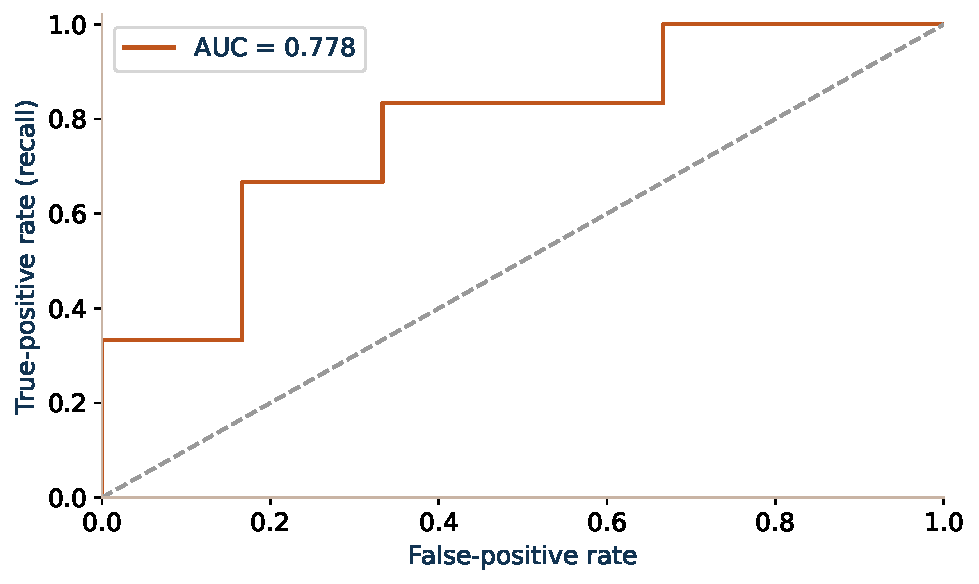
\includegraphics[width=.86\textwidth,height=.64\textheight,keepaspectratio]{figures/supervised/roc_example.pdf}\par\small ROC varies the threshold. AUC summarises ranking across positive-negative pairs, with half credit for ties.
\end{frame}

\begin{frame}{What AUC does not tell us}
\begin{itemize}
\item AUC is not accuracy at one threshold.
\item AUC does not assess whether probabilities are calibrated.
\item AUC does not encode the costs of the errors or an operational capacity limit.
\item With a rare event, also inspect precision-recall behaviour, prevalence and positive counts.
\end{itemize}
\end{frame}

\begin{frame}{Calibration}
\begin{itemize}
\item Among observations assigned probabilities near 0.20, does the event occur about 20\% of the time?
\item Compare average predicted probabilities with observed event rates in groups.
\item Show group sizes; small bins produce noisy comparisons.
\item A model may rank cases well while systematically overpredicting risk.
\end{itemize}
\end{frame}

\begin{frame}{Probability scores}
\[\text{Brier score}=\frac1n\sum_i(y_i-\hat p_i)^2.\]\[\text{Log loss}=-\frac1n\sum_i\{y_i\log\hat p_i+(1-y_i)\log(1-\hat p_i)\}.\]\begin{itemize}
\item Lower values indicate better probability predictions under these scores.
\item Log loss penalises confident incorrect predictions heavily.
\item Compare with a constant probability estimated from the training event rate.
\end{itemize}
\end{frame}

\begin{frame}{A complete evaluation workflow}
\begin{itemize}
\item Fit the logistic model using training data.
\item Choose the threshold on validation data using stated costs.
\item Freeze the model, predictors, preprocessing and threshold.
\item Evaluate test-set classification errors, probability scores, ROC and calibration.
\item Report the sampling design and limits of generalisation.
\end{itemize}
\end{frame}

\begin{frame}{Late filing as a course case}
\begin{itemize}
\item Use 600 simulated records with outcomes available for every record.
\item Predictors are measured before the filing deadline.
\item Compare error counts across digital and other filing channels as a small illustration.
\item Discuss what changes if labels are observed only for previously audited cases.
\item An estimated probability supports analysis; it does not establish wrongdoing.
\end{itemize}
\end{frame}

\begin{frame}{R laboratory}
\begin{itemize}
\item \texttt{03\_logistic\_regression.R}: fit, odds ratios, validation and evaluation.
\item \texttt{05\_tax\_compliance\_case.R}: late-filing example and group summaries.
\item \texttt{06\_trees\_optional.R}: shallow-tree comparison.
\item Use \texttt{family=binomial()} and \texttt{type="response"} for predicted event probabilities.
\end{itemize}
\end{frame}

\begin{frame}{Applied task}
\prompt{Recommend a threshold for a reminder programme. Explain the target, the error costs, the validation procedure and what evidence would be needed before real use.}\begin{itemize}
\item Report one confusion matrix with labelled axes.
\item Give recall, precision and a probability score.
\item Distinguish an odds ratio from a probability difference.
\item Explain one limitation involving labels, sampling or human decisions.
\end{itemize}
\end{frame}

\begin{frame}{Checkpoint}
\begin{itemize}
\item What does $e^{\beta_j}$ measure?
\item Why can the probability effect vary across observations?
\item Why is a high accuracy insufficient for rare-event prediction?
\item Why must threshold selection precede final test evaluation?
\item Can a well-ranked set of predictions still have poor calibration?
\end{itemize}
\end{frame}
